\chapter{ロボット制御と深層学習}
\label{chap_review}

\section{ニューラルネットワーク}\label{sec:NeuralNetwork}
人間の脳にはニューロンと呼ばれる神経細胞が1000億個以上あり,それぞれが複数のニューロンが電気信号によって情報を伝達している.また脳にはシナプスという場所があり,ここで電気信号を細胞体へ受け渡す.細胞体はある閾値以上の電気信号がきた場合に他のニューロンへ電気信号を伝播させる(これを発火と呼ぶ).このようなニューロンとシナプスで行われる演算を模倣したアルゴリズムを作ることができれば,人間のような思考や認識をコンピュータを使って再現できると考えた.そのアルゴリズムがニューラルネットワーク(Neural Network: NN)である.

\subsection{多層パーセプトロン}
ニューラルネットワークは入力層,出力層,隠れ層から構成され,層と層の間にはニューロン同士のつながりの強さを示す重みがある.非線形問題を扱うために1986年Rumelhartによって考案されたのが,パーセプトロンを複数つなぎ合わせ入力と出力以外に隠れた層を持つ多層パーセプトロン(Multi-layer perceptron: MLP)である(\fig {mlp}).ニューラルネットワークで多層パーセプトロンの層を全結合(fully connected: FC)層とも呼ぶ.

\begin{figure}[H]
	\centering
	\begin{minipage}[b]{0.4\columnwidth}
		\centering
		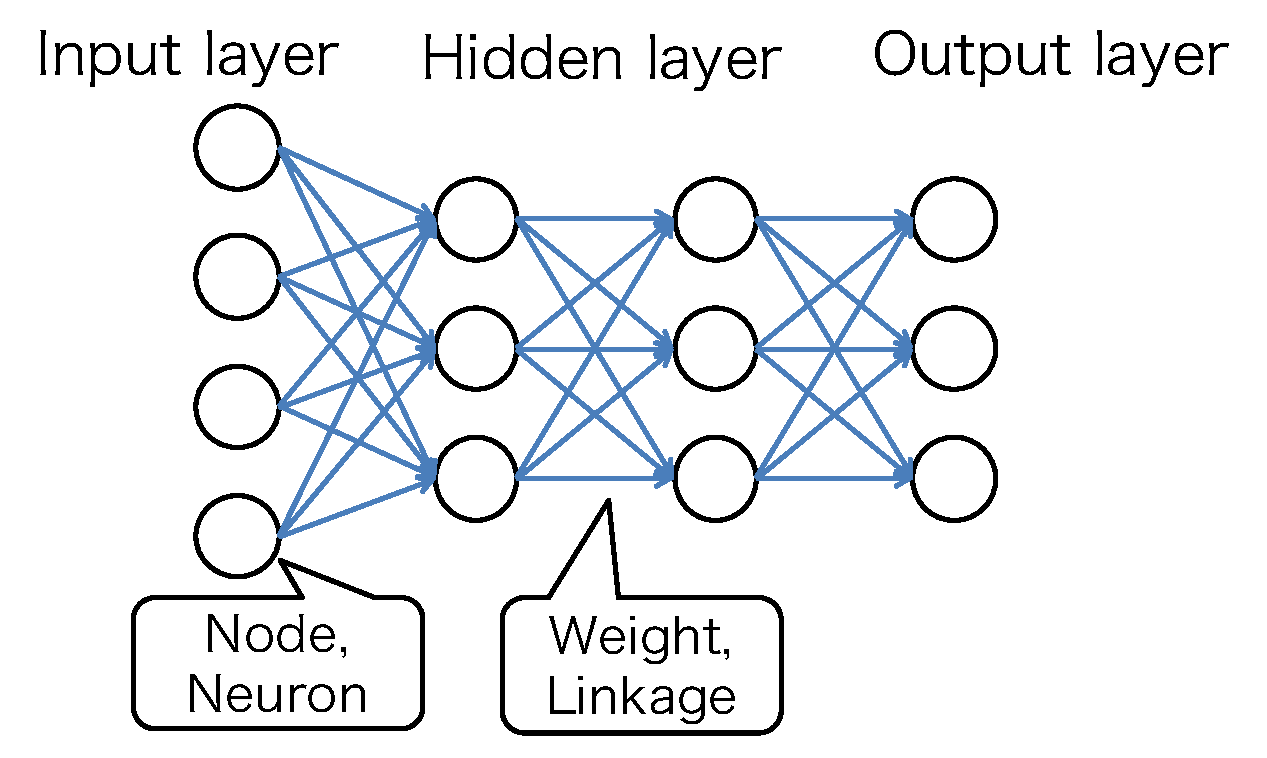
\includegraphics[width=1.2\linewidth]{fig/Review/MLP}
		\subcaption{Muti-layer perceptron}
		\label{fig:mlp}
	\end{minipage}
	\begin{minipage}[b]{0.4\columnwidth}
		\centering
		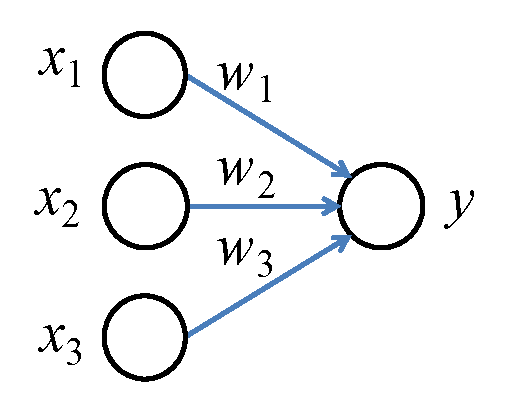
\includegraphics[width=0.7\linewidth]{fig/Review/simple_perceptron}
		\subcaption{Simple perceptron}
		\label{fig:perceptron}
	\end{minipage}
	\caption{Architecture of Muti-layer perceptron}
\end{figure}

\fig {mlp}における丸や矢印はそれぞれノード(またはニューロン)と重み(または結合)と呼び,ともに数値である.例えば画像を分類しようと思えば,各ピクセルの画素数を各ノードに入力する.例えば$28 \times 28$pxのグレースケール画像であれば,784個のノードが必要となる.入力データ$\bm {x}$が入力層に入ってくると,その値に重み$\bm {w}$をかけ,活性化関数$H$と呼ばれる関数に通し,結果$\bm{y}$を出力する.ここで,入力$\bm{x}$,重み$\bm{w}$,出力$\bm{y}$を太字で表したが,これらは全てテンソルであり,1つの層にあるノード$x_1, x_2, \cdots x_n$を一括して$\bm {x}$として表記している.

ここで,中間層の1つのノードについて考える.\fig {perceptron}にMLPを構成する1ユニットである単純パーセプトロンを示した.この模式図を数式で表すと次のようになる.
\begin{align}
	y & = H(\bm{w}\bm{x} + \bm{b}) \\
	& = H\left( \sum_{i=1}^3 w_i x_i + b_i \right) 
\end{align}
ここで$\bm{b}$はバイアスと呼ばれ,発火のしやすさを表している.中間層における活性化関数は,\eq {ReLU}に示す正規化線形関数(rectified linear unit: ReLU)と呼ばれる関数)がよく用いられる.
\begin{align}\label{eq:ReLU}
	H(x) = \max \left\lbrace 0, x \right\rbrace = \begin{cases}
	x & (x > 0) \\
	0 & (x \leq 0)
	\end{cases}
\end{align}
この演算を繰り返し出力層に書き出す.ここで,各層の重みの値によって出力結果は異なってくる.

出力層では,ノードの個数は区別したいクラス数分用意する.
各ノードの出力値が各クラスに属している確率を表すように,活性化関数にはソフトマックス関数を用いる(ただし二値分類の場合はシグモイド関数を用いる).ソフトマックス関数は\eq {softmax}で表される.
\begin{align}\label{eq:softmax}
	y_i = \dfrac{\exp(x_i)}{\displaystyle \sum_{k=1}^n \exp(x_k)}
\end{align}
ここで$y_i$は,出力層が全部で$n$個あるとして,$i$番目の出力であることを示す.\eq {softmax}からわかるように,入力の総和に対して1つのノードがどれくらいの値を持つかという割合で表されている.これにより各ノードの出力は確率として解釈できるため,値の一番大きいノードのインデックスを予測ラベルとして見ることができる.


\subsection{畳み込みニューラルネットワーク}
従来の画像認識では,画像から特徴を抽出しそれを識別器にかける手法が主流であった.古典的手法では画像から特徴を抽出するいわゆる特徴量設計が必要で,ここをいかにうまく設計するかがポイントであった.特徴抽出の方法として,HOG\cite{HOG}やSIFT\cite{SIFT},SURF\cite{SURF}などがあり,これらによって抽出した特徴ベクトルをSupport Vector Machine(SVM)\cite{SVM}によって識別することが多かった.

しかし,1998年にLeNetと呼ばれる畳み込みニューラルネットワーク(Convolutional Neural Network: CNN)が提案された\cite{LeNet}.CNNは畳み込み層とプーリング層からなっている.この畳み込みとプーリングの演算を通して,特徴量設計から識別までをend-to-endで行うことができる.

\begin{figure}[H]
	\centering
	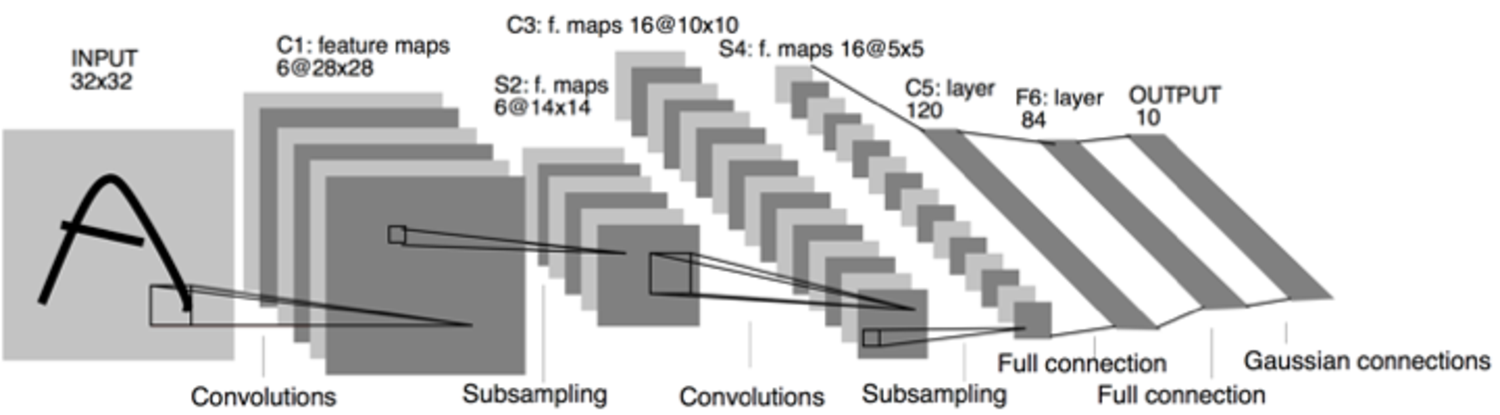
\includegraphics[width=0.7\linewidth]{fig/Review/LeNet}
	\caption{Architecture of convolutional neural network\cite{LeNet}}
	\label{fig:LeNet}
\end{figure}


%人間が物体を認識することをコンピュータにも計算させるには,画像の特徴的な部分を切り分けて数値化させる必要がある.例えば,カラー画像の場合,RGBの3色(3チャンネル)を組み合わせた画像で認識をしている.このようなフィルターの畳み込み計算を行うと,フィルターごとに異なった画像の特徴を抽出して数値化する.これが畳み込み(convolution)である.その後,画像のサイズを小さくしてコンピュータが計算コストを減らし,微小な変化に対してロバストになる仕組みしてプーリングという方法を用いる.

畳み込み層では,入力に対してフィルター(カーネルとも呼ばれる)を用意し,\eq {conv}に示す計算を行う.
\begin{align}\label{eq:conv}
	y_{i,j} & = (\bm{K} * \bm{x})_{i,j}\\
	& = \sum_m\sum_n x_{i+m, j+n} K_{m,n}
\end{align}
ここで,$\bm{K}$はフィルター,$\bm{x}$は入力,$y$は出力である.CNNではこの演算の後に活性化関数に通す.これを図で表すと\fig {conv}のようになる.

\begin{figure}[H]
	\centering
	\begin{minipage}{0.45\columnwidth}
		\centering
		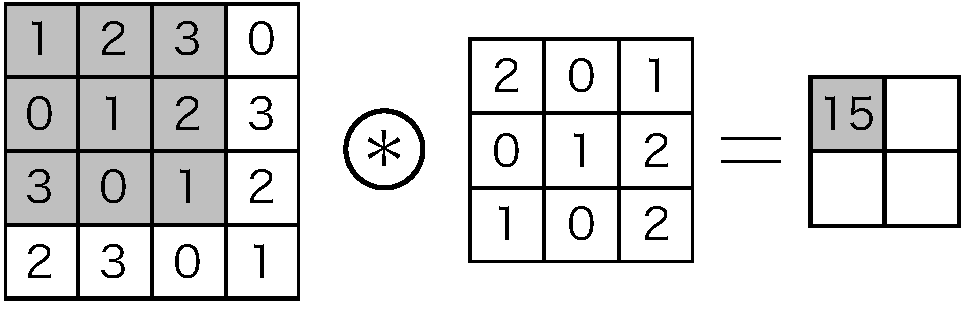
\includegraphics[width=\linewidth]{fig/Review/conv_ex1}
		\subcaption{}
		\label{fig:conv_ex1}
	\end{minipage}
	\hspace{10truemm}
	\begin{minipage}{0.45\columnwidth}
		\centering
		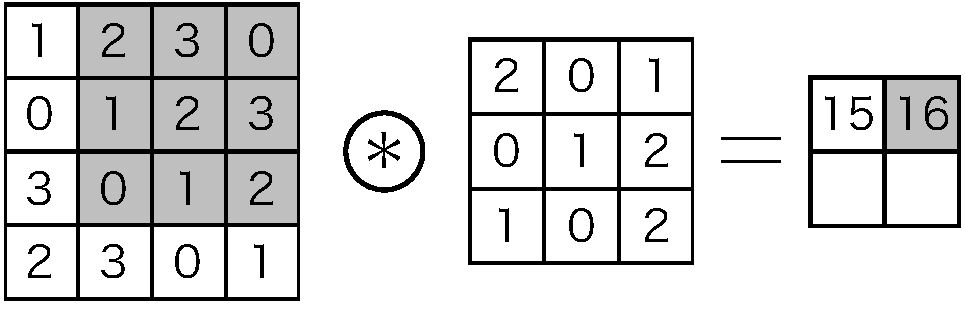
\includegraphics[width=\linewidth]{fig/Review/conv_ex2}
		\subcaption{}
		\label{fig:conv_ex2}
	\end{minipage}
	\begin{minipage}{0.45\columnwidth}
		\centering
		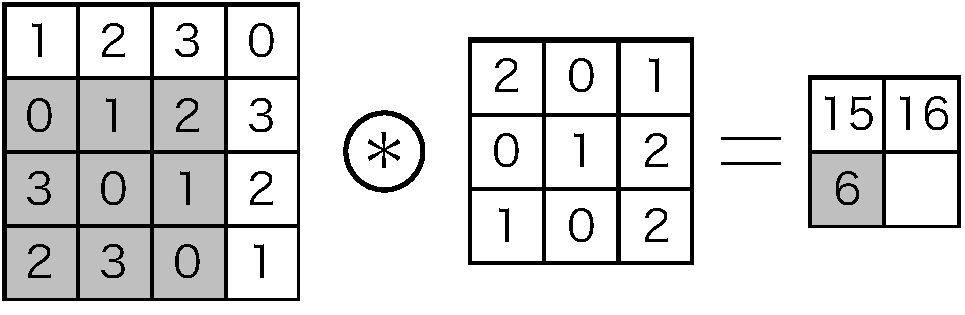
\includegraphics[width=\linewidth]{fig/Review/conv_ex3}
		\subcaption{}
		\label{fig:conv_ex3}
	\end{minipage}
	\hspace{10truemm}
	\begin{minipage}{0.45\columnwidth}
		\centering
		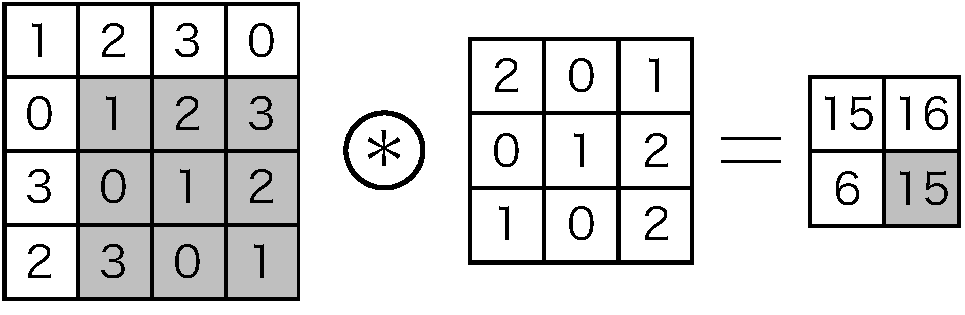
\includegraphics[width=\linewidth]{fig/Review/conv_ex4}
		\subcaption{}
		\label{fig:conv_ex4}
	\end{minipage}
	\caption{Operation process of convolution}
	\label{fig:conv}
\end{figure}

\fig {conv}では,フィルターのサイズは$3\times 3$であるが,大きさは任意である($3\times 3$や$5\times 5$, $7\times 7$がよく用いられる).また,フィルターは1マスずつ横にずらして計算を行っている.ずらし方をストライドといい,今回はストライド1である.CNNでは多くの場合,ストライドは1である.
このようなフィルターの畳み込み計算を行うと,フィルターごとに異なった画像の特徴を抽出して数値化することができる.

次にプーリングを行う.ここでは,画像認識で多く用いられる最大値プーリングについて述べる.\fig {maxpooling}に示すように,$2\times 2$のプールサイズを用意した時,その範囲内にある最大値を取る演算である.ストライドはプールサイズと合わせ,プーリングを行った領域と被らないようにすることが一般的である.\fig {maxpooling}ではストライド2である.

\begin{figure}[H]
	\centering
	\begin{minipage}[b]{0.4\columnwidth}
		\centering
		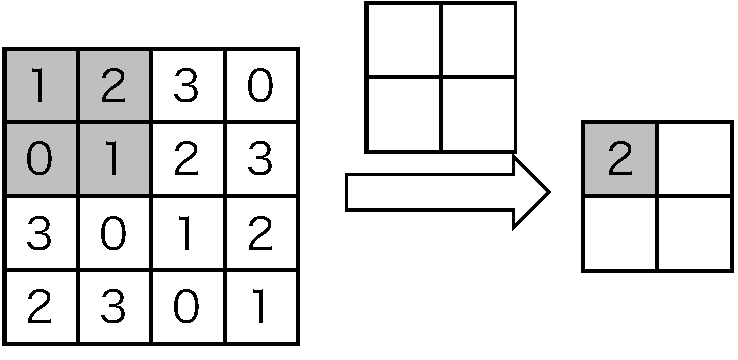
\includegraphics[width=\linewidth]{fig/Review/pooling_ex1}
		\subcaption{}
		\label{fig:pooling_ex1}
	\end{minipage}
	\hspace{10truemm}
	\begin{minipage}[b]{0.4\columnwidth}
		\centering
		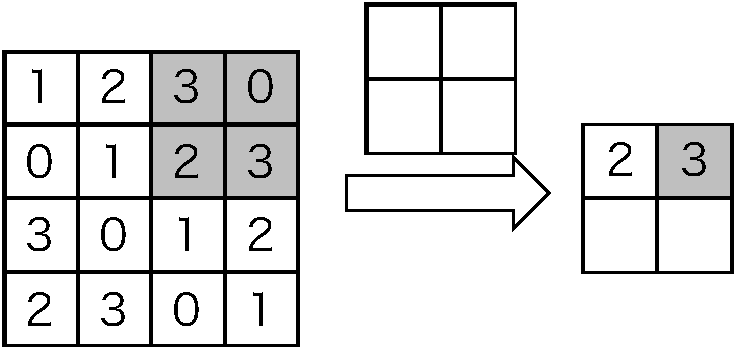
\includegraphics[width=\linewidth]{fig/Review/pooling_ex2}
		\subcaption{}
		\label{fig:pooling_ex2}
	\end{minipage}
	\begin{minipage}[b]{0.4\columnwidth}
		\centering
		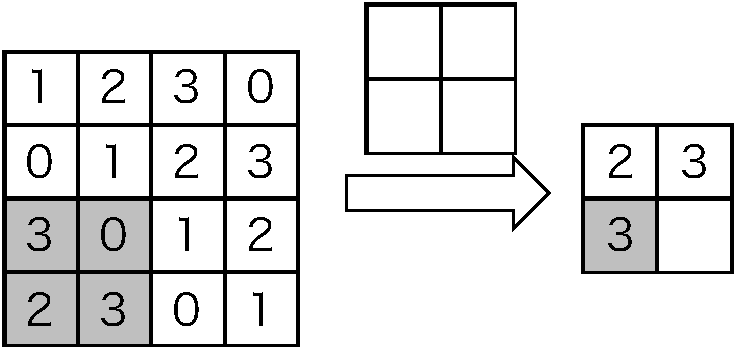
\includegraphics[width=\linewidth]{fig/Review/pooling_ex3}
		\subcaption{}
		\label{fig:pooling_ex3}
	\end{minipage}
	\hspace{10truemm}
	\begin{minipage}[b]{0.4\columnwidth}
		\centering
		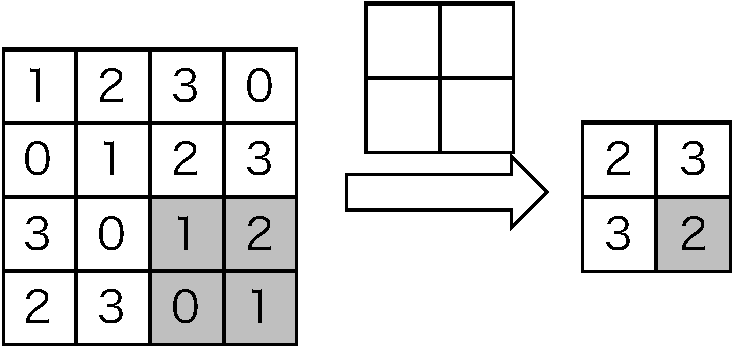
\includegraphics[width=\linewidth]{fig/Review/pooling_ex4}
		\subcaption{}
		\label{fig:pooling_ex4}
	\end{minipage}
	\caption{Operation process of max pooling}
	\label{fig:maxpooling}
\end{figure}

プーリング層では画像のサイズを小さくして(コンピュータの)計算コストを減らし,微小な変化に対してロバストになる.

この畳み込みとプーリングを繰り返して,入力からフィルターの数だけ特徴を抽出し,この抽出した特徴マップをFC層へ繋げて識別を行う手法がCNNである.


\section{推論と学習}
ニューラルネットワークでは推論フェーズと学習フェーズに分かれている.\ref{sec:NeuralNetwork}節は全て推論フェーズの話であり,順伝播ニューラルネットと呼ばれる.

学習フェーズでは,逆伝播ニューラルネットを用いる.逆伝播とは誤差逆伝播法(Backpropergation)\cite{Backprop}から由来している.真値からの誤差を表す損失関数(loss function)を用いて,パラメータの微分値を更新に用いる.損失関数はコスト関数,目的関数とも呼ばれる.この微分値を効率よく計算するアルゴリズムが誤差逆伝播法である.

損失関数は解く問題の目的に合わせて選ぶ必要がある.回帰問題では平均二乗和誤差(mean squared error: MSE)が用いられる.
\begin{align}\label{eq:mse}
	L_{\mathrm{MSE}} = \dfrac{1}{2} \sum_{k} (y_k - t_k)^2
\end{align}
また,クラス分け問題では交差エントロピー誤差(cross entropy error)が用いられる.
\begin{align}\label{eq:crossentropy}
	L_{\mathrm{cross}} = - \sum_k t_k \ln {y_k}
\end{align}
ここで,$y$は予測ラベルで,$t$は教師ラベルである.

\subsection{最適化手法}
損失関数を用いてパラメータを更新するが,更新手法にはいくつか方法があるため,ここでは本研究で使用した最適化手法について述べる.

\subsection*{SGD}
SGDは日本語で確率的勾配降下法(Stochastic gradient descent)と呼ばれる手法で,最も単純な最適化手法である.画像認識の分野では多く使われている.

SGDでは以下の式\eq {SGD}でパラメータを更新する.
\begin{align}\label{eq:SGD}
	\bm{W} \leftarrow \bm{W} - \eta \pdif{L}{\bm{W}} 
\end{align}
ここで,$\bm{W}$は更新する重みパラメータ,$\pdif{L}{\bm{W}}$は$\bm{W}$に関する損失関数の勾配である.また$\eta$は学習率と呼ばれ,実際には0.01や0.001といった値を前もって決めて使用する.SGDはパラメータの勾配を利用して,勾配方向にパラメータを更新するステップを繰り返して,徐々に最適なパラメータへと近づける手法である.

\subsection*{Adam}
Adam\cite{Adam}はadaptive moment estimationの略で,勾配の値の1乗和と2乗和の両方をパラメータ更新に用いる手法である.以下の式\eq{adam}でパラメータを更新する.

\begin{align}\label{eq:adam}
	\bm{m} & \leftarrow \beta_1 \bm{m} + (1 - \beta_1) \pdif{L}{\bm{W}} \\
	\bm{v} & \leftarrow \beta_2 \bm{v} + (1 - \beta_2) \left( \pdif{L}{\bm{W}} \right) ^2 \\
	\bm{W} & \leftarrow \bm{W} - \eta \dfrac{\hat{\bm{m}}}{\sqrt{\hat{\bm{v}}} + \epsilon} 
\end{align}

$m_t$と$v_t$はそれぞれ、勾配の一次モーメント(平均値)と二次モーメント(分散した平方偏差)の概算値である.$\eta$,$\beta_1$,$\beta_2$はそれぞれ学習パラメータである.
また,$\hat{m}_t$,$\hat{v}_t$はそれぞれ移動指数平均を用いた際に生じるバイアス(大きさを変えてしまっていることなど)を打ち消すために正則化しており,\eq {adamhat}で表される.

\begin{align}\label{eq:adamhat}
	\hat{\bm{m}} & = \dfrac{\bm{m}}{1 - \beta_1} \\
	\hat{\bm{v}} & = \dfrac{\bm{v}}{1 - \beta_2}
\end{align}

学習パラメータはそれぞれ$\eta = 0.001$,$\beta_1 = 0.9$,$\beta_2 = 0.999$,$\epsilon = 10^{-8}$が最適だと言われている\cite{Adam}.

\subsection{学習のテクニック}
ディープラーニングでは過学習(overfitting)と呼ばれる問題が多く起こる.過学習とは,訓練データに対してのみ適応し過ぎてしまい,訓練データに含まれないテストデータには精度が出ない状態を指す.過学習は,大量にパラメータを持つ表現力の高いモデルであることや,訓練データが少ないことなどが原因で起こる.ここでは過学習を抑制するテクニックを述べる.

\subsection*{Dropout}
Dropout\cite{Dropout}は,ネットワークのノードをランダムに消去しながら学習する手法である.訓練時に隠れ層のノードを毎回ランダムに選択し,そのノードの出力を0にする.そしてテスト時には全てのノードを活性化させ,信号を伝達させる.

Dropoutは,学習時にノードをランダムに消去することで,毎回異なるモデルを学習していると解釈でき,アンサンブル学習と同じ効果を擬似的に1つのネットワークで実現していると考えられる.アンサンブル学習とは,弱識別器を複数合わせて1つの強力な識別器とする手法で,現在でも有効な手法として用いられている.

\subsection*{Batch Normalization}
Batch Normalization\cite{BatchNorm}は,ネットワークにおける各層での活性化後の出力(アクティベーション)の分布を,適度な広がりを持つように調整する手法である.Batch Normalizationでは学習を行う際のミニバッチを単位として,ミニバッチごとに正規化を行う(\eq {BatchNorm}).
\begin{align}\label{eq:BatchNorm}
	\mu_B & = \dfrac{1}{m}\sum_{i=1}^m x_i \\
	\sigma_B^2 & = \dfrac{1}{m}\sum_{i=1}^m (x_i - \mu_B) \\
	\hat{x_i} & \leftarrow \dfrac{x_i - \mu_B}{\sqrt{\sigma_B^2 + \epsilon}}
\end{align}
ミニバッチとして$B = \{x_1, x_2, \cdots, x_m\}$という$m$個の入力データの集合に対して,平均$\mu_B$,分散$\sigma_B^2$を求め,入力データを平均0分散1となるように正規化を行う.$\epsilon$は0で除算されることを防ぐもので,極小の値を用いる.

Batch Normalizationを用いると,学習を速く進行させることができる,初期値にそれほど依存しない,過学習を抑制できるといった効果が期待できる.

\subsection*{Data Augumentation}
Data Augumentation(データ拡張)は,訓練データを人工的に水増しする手法である.例えば,入力画像に対して回転や縦横の移動,上下反転,鏡面反転などの操作をして訓練データを擬似的に増やす.これは,ニューラルネットは大きな位置ずれや対象物が回転した状態にあると別のものとして認識してしまうことを逆手にとった手法である.訓練データが少ないときに大きな効果を発揮する.


\section{機械学習の評価指数}
機械学習の評価のために,混同行列(Confusion Matrix)を用いる.\fig{confusionmatrix}で真のクラスと予測クラスに分かれて,PositiveとNegativeは今回のような病理診断の場合は,正常と腫瘍に対応する.したがって,True PositiveとTrue Negativeは,正常の画像を正常と正しく判定し,腫瘍の画像を腫瘍と正しく判定したという意味である.そしてFalse Positiveは,本当は正常の画像を,腫瘍であると間違って判定することである.最後にFalse Negativeは,本当は腫瘍の画像であるものを正常と間違って判定すること,つまり腫瘍を見落としたということになる.見落としを防止するためにはFalse Negativeがゼロになるような診断アルゴリズムを開発することが重要になる.

\begin{figure}[H]
    \centering
    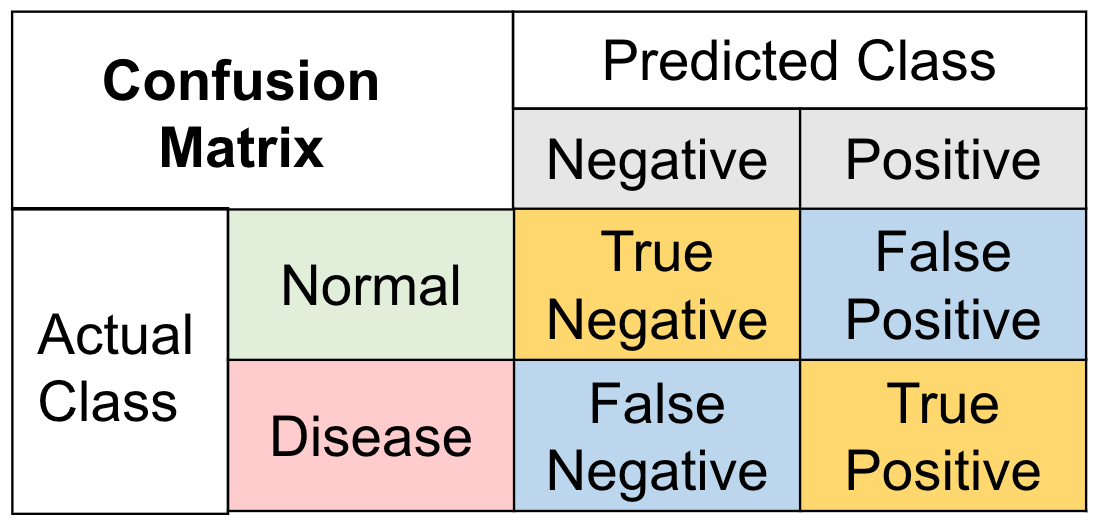
\includegraphics[width=0.7\linewidth]{fig/Review/confusion_matrix}
    \caption{Confusion matrix}
    \label{fig:confusionmatrix}
\end{figure}

\begin{figure}[H]
    \centering
    \begin{minipage}{0.7\columnwidth}
        \centering
        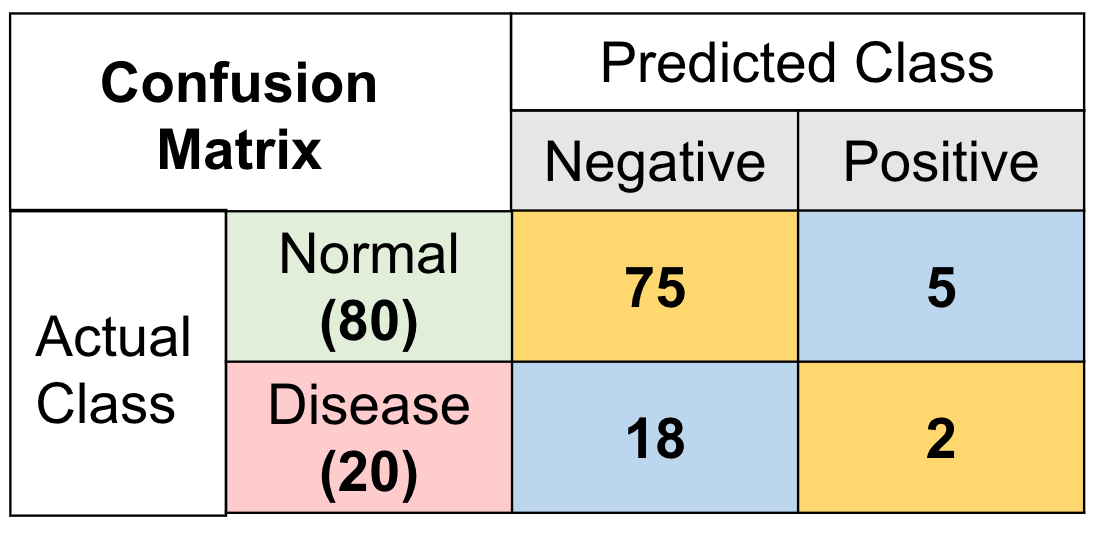
\includegraphics[clip, width=0.7\linewidth]{fig/Review/confusion_examples}
        \subcaption{Example of Confusion matrix table}
        \label{fig:confusion_table}
    \end{minipage}
    \begin{minipage}{0.9\columnwidth}
        \centering
        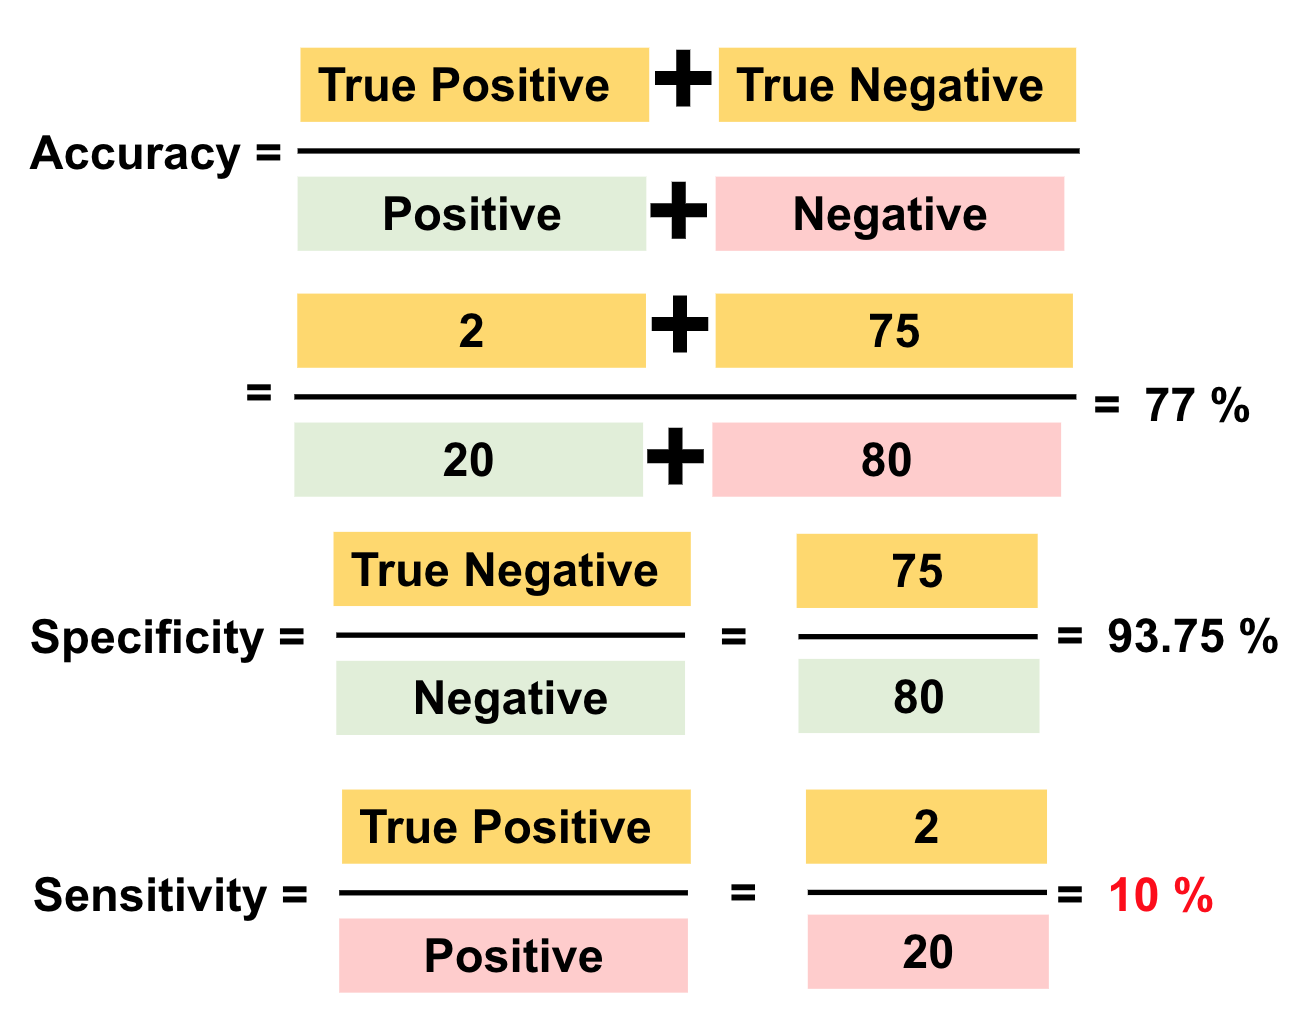
\includegraphics[clip, width=0.7\linewidth]{fig/Review/confusion_math}
        \subcaption{Accuracy and Sensitivity and Specificity}
        \label{fig:confusion_math}
    \end{minipage}
    \caption{Example of Confusion matrix}
    \label{fig:confusion_ex}
\end{figure}

機械学習による病理診断アルゴリズムを評価するために,3つの指標がある.AccuracyとSpecificty(特異度)とSensitivity(感度)である.なぜ,Accuracyだけではなく,SensitivityとSpecificityが必要かを説明する図が\fig{confusion_ex}である.この場合だとAccuracyが8割弱で良いと判断することもできるが,Sensitivityに注目すると1割しかないので,この機械学習のモデルでは,腫瘍の画像を腫瘍であると認識することができていないことが分かる.見落とし防止を目標にする場合は,Sensitivityが重要な指標になる.

\begin{figure}[H]
    \centering
    \begin{minipage}{0.8\columnwidth}
        \centering
        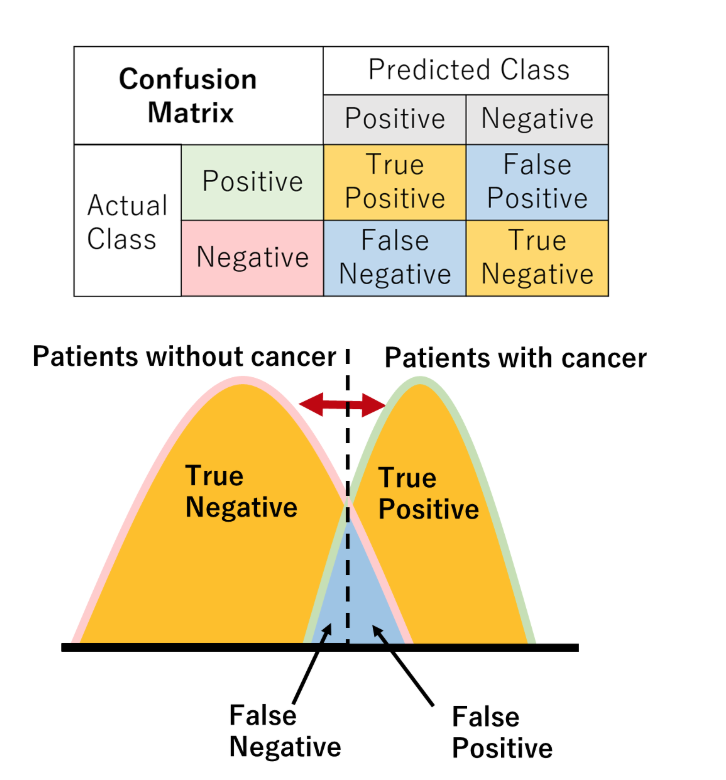
\includegraphics[clip, width=0.7\linewidth]{fig/Review/why_roc}
        \subcaption{How to get ROC curve}
        \label{fig:why_roc}
    \end{minipage}
    \begin{minipage}{0.6\columnwidth}
        \centering
        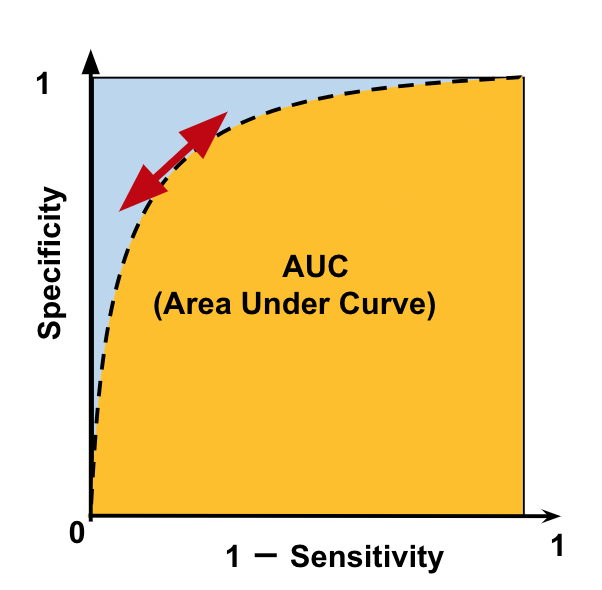
\includegraphics[clip, width=0.7\linewidth]{fig/Review/roc_curve}
        \subcaption{ROC Curve}
        \label{fig:roc_curve}
    \end{minipage}
    \caption{ROC Curve and AUC}
    \label{fig:roc}
\end{figure}

機械学習を使って推論を行うとき,正常と腫瘍の確率が出る.これを50\%を閾値にして,判定するのではなく,例えば目的に応じて40\%の確率で腫瘍と認識される場合も腫瘍と判定するというように閾値を変更することで,判定結果をSensitivityが高くなるように,またはSpecificityが高くなるように変動させることができる.(\fig{why_roc})
このように閾値を変化させるときに,変化するSensitivityとSpecificityをプロットしていくと\fig{roc}の点線のような値をとる.これをReceiver Operating Characteristic(ROC)曲線と呼び,機械学習の性能評価で用いられる.また,点線の内側の面積をArea Under Curve(AUC)と呼び,この値を評価指数として利用する.


\section{画像認識と深層学習}
Deep LearningとはDeep Neural Network(DNN)を指すことが多い.この"Deep"とは,ニューラルネットワークの層が深いことに由来している.

\fig {ImageNet}に画像認識タスクの精度の近年の推移を示す.これはImageNet Large Scale Visual Recognition Challenge (ILSVRC)と呼ばれる世界的な画像認識のコンペティションである(2010年から始まった).カテゴリ数は1000クラスで,画像枚数は120万枚の訓練データと15万枚のテストデータが用意されている.
\begin{figure}[H]
	\centering
	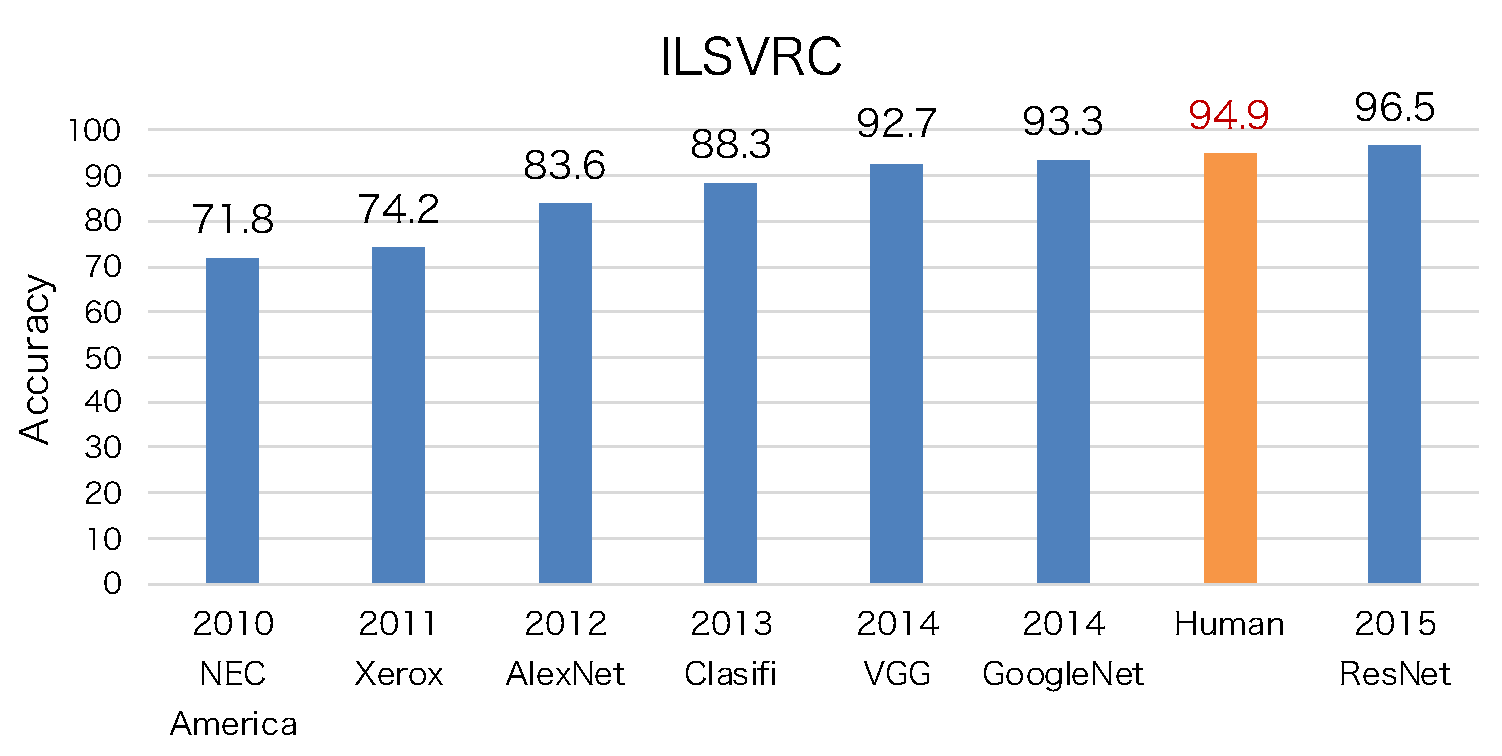
\includegraphics[width=0.7\linewidth]{fig/Review/ILSVRC}
	\caption{Transition of accuracy of image recognition on ILSVRC}
	\label{fig:ImageNet}
\end{figure}
2011年と2012年は約10\%もの大差でAlexNet\cite{AlexNet}が優勝している.これがディープラーニングの始まりである.AlexNetは5つの畳み込み層と3つの全結合層を持っている.2014年にはVGGNet\cite{VGGNet}やGoogLeNet\cite{GoogLeNet}が9割の精度を超えた.VGGNetはAlexNet(8層)よりさらに深い構造(19層)であり,GoogLeNetは22層もある.そして2015年にはResNet\cite{ResNet}が人間の精度をも超える認識精度を達成した.ResNetはGoogLeNetよりもさらに深く152層もある.CNNを複数回かけて検出を行う場合,CNNの浅い側では空間分解能はあるが抽象的な情報が少ない.深い側では意味論的な情報は取得できる(ポーズ,変形など)が空間分解能が小さいため幾何学的な情報が失われる.

アーキテクチャの進化の方向は大きく3つある.1つ目は層を深くすることである.2つ目はFC層の使用を避ける,またはInceptionモジュールの使用することである.これにより学習するパラメータ数を削減することができる.3つ目はResNetなどのショートカット接続の利用や,事前学習・転移学習を行うことである.これによって学習効率を向上させ,最終的にモデルの精度向上へと繋がる.ここで,事前学習のデータセットと適用データとの間には類似性があると良い.

画像処理におけるディープラーニングでは大きく3つのタスクがあり,それぞれ,クラス分類,物体検出,セグメンテーションである.以下に詳細を述べる.

\subsection*{クラス分類}
クラス分類は画像に写っている物体が「dog」「airplane」「bird toy」など事前に定義されたラベルのどれが適切かを識別するタスクである.この識別は,事前に定義されたラベルの特徴べクトルと入力画像の特徴べクトルの距離計算を行い,距離値が小さければ同一,そうでなければ否と判定する.指紋照合,顔照合,人物照合では,本人と他人を判定するタスクとなる.深層学習では,同一人物のペア画像間の距離値が小さく,他人の画像との距離値が大きくなるような損失関数を設計し,ネットワークを構築することで人物照合問題を解いている.

\subsection*{物体検出}
物体検出とはBounding Boxで物体の位置とその物体の種類を特定する方法である.歴史的には幾何的情報,手動特徴量,そしてそのカスケードを利用していた.その後,HOG\cite{HOG}やSIFT\cite{SIFT}など局所特徴量を抽出する方法を設計するようになったが,これは深い専門知識を必要とした.また広い範囲でオブジェクトを正確に検出する方法は,メモリ容量と処理時間に課題がある.現在はDeep Neural Networkが主流となり,データのみから抽象的な特徴量を複数得ることができる.\fig {SSD}に物体検出で有名はアルゴリズムであるSSD\cite{SSD}とYOLO\cite{YOLOv3}のアーキテクチャを示す.クラス分けの場合は数1000のカテゴリを学習してTop Error Rateが2\%以下と人間よりも認識精度が高いが,物体検出においては,現状ではカテゴリが数100程度くらいまででも認識精度が人間よりも低くなってしまう.また物体検出は精度を上げるために処理に時間がかかることが多いため,リアルタイムに物体検出を行う時は,速度と精度のトレードオフが生じてしまう.

\begin{figure}[H]
	\centering
	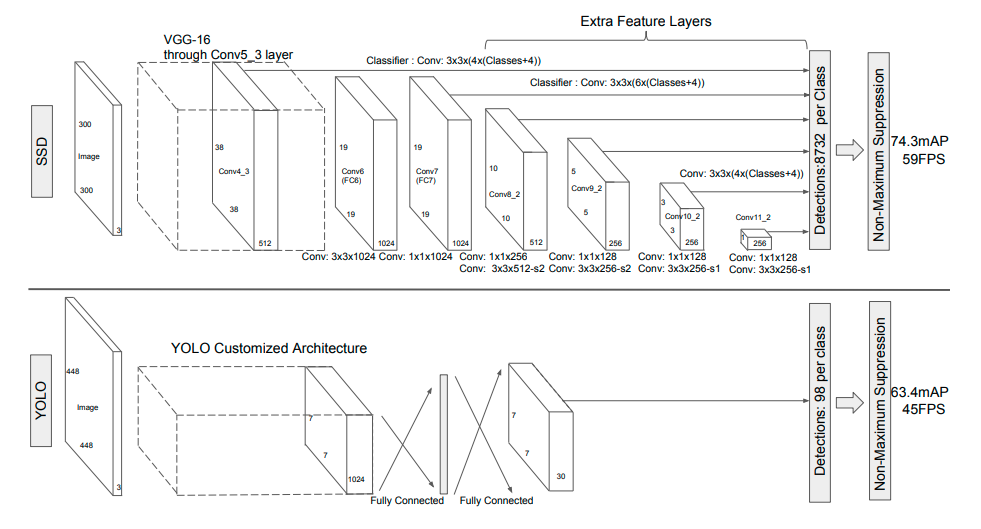
\includegraphics[width=0.7\linewidth]{fig/Review/yolo_ssd.png}
	\caption{Network Architecture of SSD and YOLO\cite{SSD}}
	\label{fig:SSD}
\end{figure}

\subsection*{セグメンテーション}
セマンティックセグメンテーションとは,画像を画素レベルで認識することである.画像内の各画素をオブジェクトクラスに割り当てる手法である.セマンティックセグメンテーションの手法についてディープラーニング以前では,Texton Forests\cite{shotton2008semantic}や,Random Forests\cite{kontschieder2011structured}に基づいた分類を行っていたが,物体検出と同様にCNNが登場してからは,高精度なセグメンテーションが実現するようになった.CNNを使ったセグメンテーションの手法で一般的に使われるようになったものがUnetである\cite{Unet}.このUnetは文字通りUの形をしたネットワークであることが特徴で,2つのアーキテクチャーからできている(\fig {Unet}).1つ目がエンコーダーのアーキテクチャーでCNNとプーリングで特徴を抽出しながら次元を削減していき,2つ目のデコーダーのアーキテクチャーで画像をセグメンテーションの結果になるように復元する.ここで問題になることが,プーリングをすることで位置情報を消してしまっているので,この位置情報を利用して画像を復元するためには,エンコーダーとデコーダーで画像サイズが同じところ同士をショートカットで接続することがUnet構造の優れている点である.

\begin{figure}[H]
	\centering
	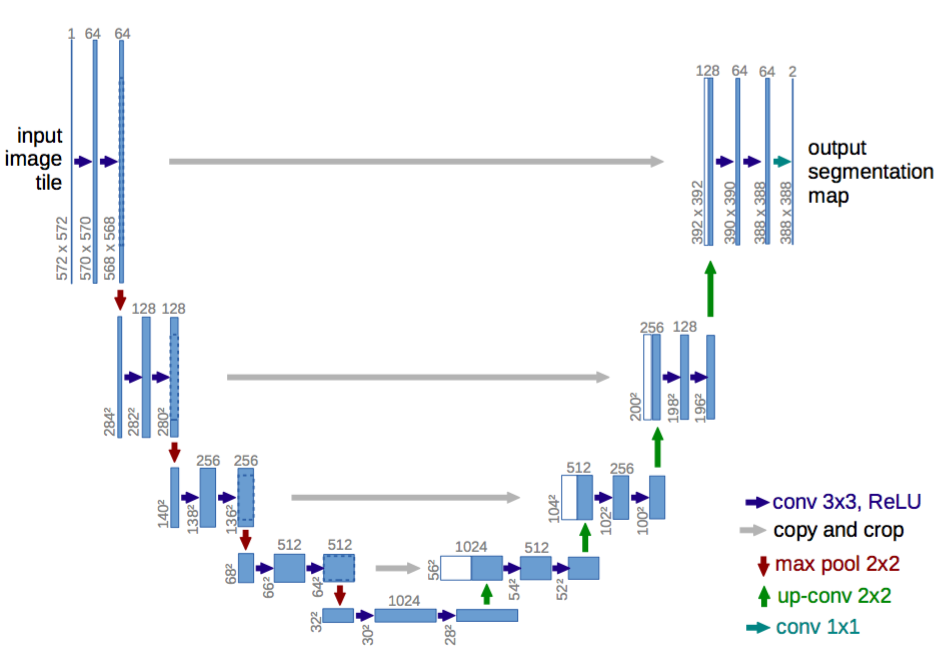
\includegraphics[width=0.7\linewidth]{fig/Review/unet.png}
	\caption{Artchitecture of Unet\cite{Unet}}
	\label{fig:Unet}
\end{figure}


\section{強化学習}


